\title{CS4731 - Project 3 Write-Up}
\author{John Rafferty \and Stephen Whipple}
\documentclass[12pt]{article}

\usepackage{parskip}
\usepackage{graphicx}

\begin{document}
\maketitle
\section{Instructions}

This project has been tested using OpenJDK Runtime Environment (IcedTea7 2.1.7) (7u3-2.1.7-1) and Apache Ant(TM) version 1.8.2.  They must be installed in order to compile and run the project.

First extract the zip entirely and open that location in a shell.

To compile this project:

\texttt{ant}

To run this project:

\texttt{ant play}

To run the project with only elevations:

\texttt{ant play-nohazards}

To clean the build files:

\texttt{ant clean}

To clean the build files and cache (warning -- next run will take a while to re-build the cache, and use a lot of Wolfram$\vert$Alpha API requests):

\texttt{ant squeakyclean}

\section{Approach}

The algorithmic approach we used in our project was to use Google Maps as our ``expert'' for generating the heights of our levels.  Because the elevations of land change in a predictable way (and they don't vary wildly between several miles), we were able to query the elevations of 50 GPS coordinates between two designated cities to get the incremental changes in elevation between the target cities.

In addition, we used Wolfram$\vert$Alpha as the method for generating additional features of our levels, based on qualities that the locations have in the real world.  For example, we base the number of coin blocks in each level on the per capita income of the population of the city nearest to the GPS location.  We also do this mapping for relative crime rate to number of enemies (and difficulty of them), for population density to the number of pipes (representing an urban area), and for number of lakes in the state to the number of pitfalls in the map.

We use probabilities with bounds checking to generate the level -- maps with a high probability for enemies but low probability for pitfalls will almost always generate a map that resembles the intended one.  We did testing and slight tweaks to ensure things like tens of blocks couldn't be placed horizontally to each other, and no jump can be too high for the player to make, but have the target set to whatever values were found by Google Maps and Wolfram$\vert$Alpha.

Our method of generation is to first create the entire map using the values that we retreive from Google Maps.  We then randomly create sections from left to right based on the actions that the player chose in the last game (the sections have their own unique characteristics).  Our game attempts to make the player have ``the most fun'' possible by tailoring the locations selected. For example, if the player gets killed by enemies often, it will choose a location that has low crime rate, and thus fewer enemies.  If the player enjoys collecting coins, it will choose a location that has a higher per captia income.

\section{Challenges}
The primary challenges that we faced dealt mostly with trying to ensure that, when the sections were generated, there could be no combination that results in an unplayable map, yet there needed to be enough variability to keep the map interesting.  Since each section was in its own class and should remain independent of the other sections (for example if another section was added or removed, other sections should not suffer -- a pluggable design that could change as more Wolfram$\vert$Alpha or Google Maps variables are added).  Another challenge that we faced dealt with the tons of queries that we'd need to perform when generating new coordinates.  If we were to take two coordinates that were very far away from each other, the 50 points that were generated between these two coordinates would likely be in different cities or states.  When modeling things like population density or crime rate, each of these required a lookup to Wolfram$\vert$Alpha.  This could potentially lead to numbers such as 200 queries if they were all in different locations, and at 1-3s to return the result, this takes forever to load.   Our solution was to implement a cache system (SQLite so that we could lookup based on different variables, like latitude and longitude or city name), which aims to bring the number of queries to Wolfram$\vert$Alpha down to zero for subsequent accesses to the same city.  It may not be exactly zero if the coordinates are different; they still require the one lookup to find the closest city -- and if we have that city cached, we can use all cached values from then on.  In addition, instead of using all 50 points to act as variable in the map, we just take the average of the source and end point for all other variables than elevation, since their variability doesn't matter as much, and it eats up all of our Wolfram$\vert$Alpha API query quota if we run it more than a few times with 50 points for each source and destination.

\section{Goal}
Our goal for the project is to create a pluggable Mario PCG library that can be fed different GPS coordinates and generate terrain based on the region that makes up the straight line distance between them.  This allows the player to be able to select familiar places to act as the Mario environment.  In addition, we selected areas that have certain properties that are mapped from how the player plays.  An example of this might be that if the player is killed in the last game by enemies, the next map will be one of the pre-generated locations that was designed to have a lower population than normal (so there are less enemies in the subsequent map).  We only look at the previous game to determine the next map, since this is easy to test and support was provided natively by the game engine (results from the last game overwrite the previous).  We find this effective to measurably demonstrate how the level changes as well as it working well for changing players or skill level by the player over time.

\section{Results}
Our approach works fairly well and the granularity provided by Google Maps for determining elevation works great.  Some of the things that we tested include the bottom of Freshman Hill to the Student Center (there is a gradual rise from the bottom of the map to the top, then the stairs that go down sharply about half way from the top are easily recognizable), and the football stadium (the silhoutte of the stadium is visible).

One cool thing that we found about basing our elevations on the geography of real places is that as long as the sampling rate is decent the generated maps always have a ``sloping'' feel to them -- they are not jagged with dramatic heights that go up then down over the course of a screen width, which would make them feel incoherent.

\section{Examples}
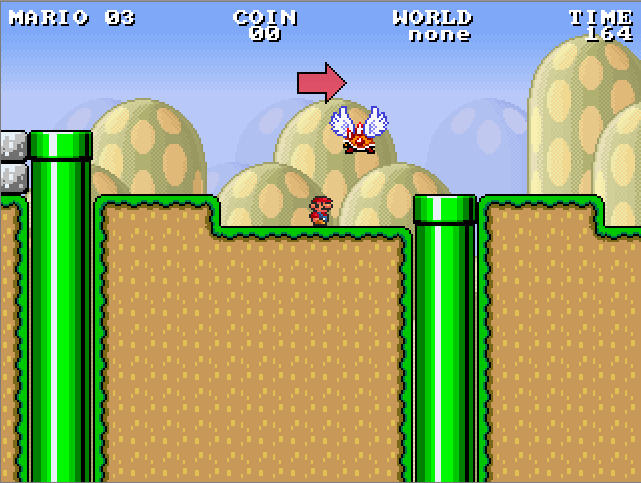
\includegraphics[width=80mm]{Mario1.png} \\
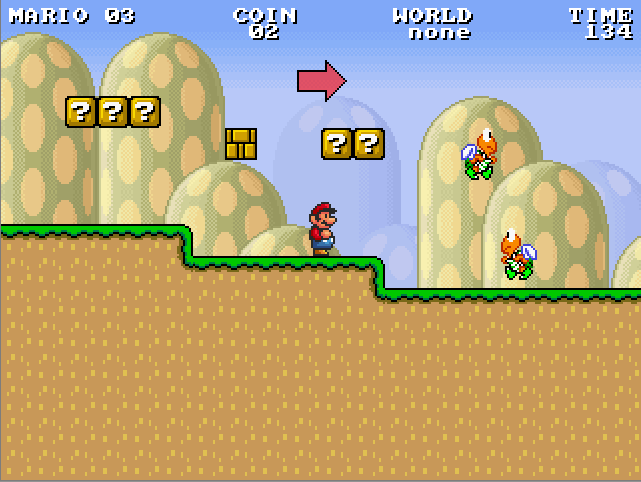
\includegraphics[width=80mm]{Mario2.png} \\
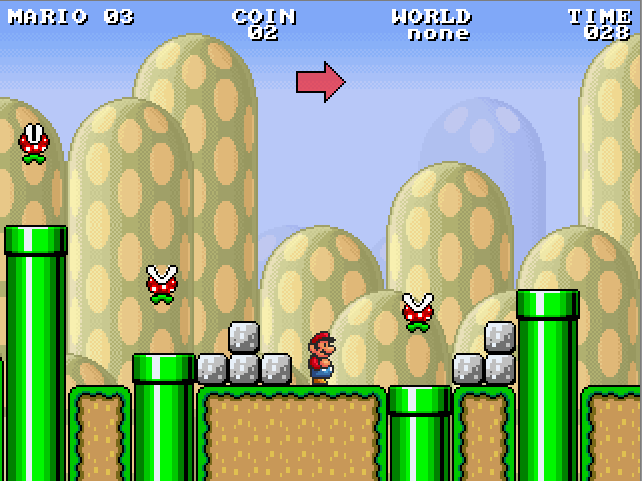
\includegraphics[width=80mm]{Mario3.png} \\
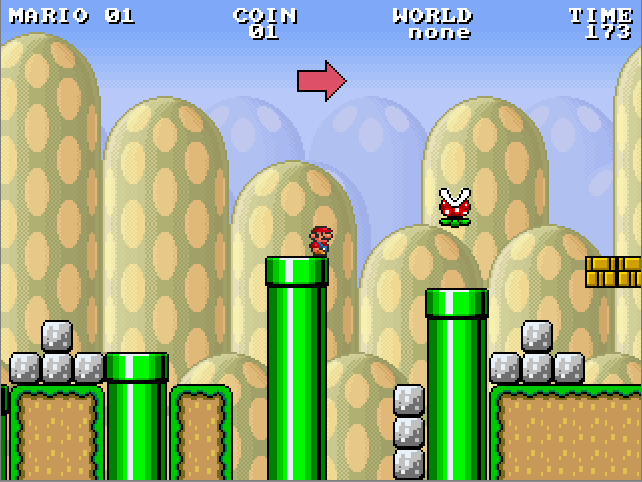
\includegraphics[width=80mm]{Mario4.png} \\

\end{document}
